\chapter{Interactive Perception Library}
\label{chapter:Interactive Perception Library}


\section{Motivation and Goals}
Based on the increasing popularity of the interactive perception approach we created a common place that can unite other people' efforts towards better algorithms and systems that concern adding manipulation in the perception loop. Since we understand the world based on functionality and behavior, as a result, manipulation becomes an integral part of perception. In other words, purposeful manipulation depends on the robot's ability to curiously explore its unknown environment through interaction. 

It is worth emphasising and it has been shown in the \ref{chapter:Related Work} that interactive perception field has gained many more potential applications than the ones presented in this thesis. These areas include interactive perception methods for object segmentation, modeling, grasping, and even learning manipulation skills through interactive perception. Interestingly, these results are beginning to appear independently in the different relevant communities: perception, grasping, manipulation, and learning.

Having this in mind we created a common, modular tool - Interactive Perception Library \footnote{\url{http://github.com/Lolu28/interactive_perception}} that can address researchers' needs to investigate interactive perception area more deeply and it can enable easier access to existing resources and algorithms. The main goal of this library is to collect all the code from different laboratories being involved in the idea of interactive perception. We came up with a framework that enables to switch between different implementations of each step from the interactive perception pipeline at runtime. 


\section{Library}
\subsection{Steps}
Looking at various systems created by different robotics institutes REF it can be noticed that there is a similar idea lying behind them.  

After conducting research in existing implementations we noticed many similar steps that became crucial for our library, those being:

\begin{itemize}
\item Static Segmentation - to infer which parts of the scene are most likely being segmented incorrectly
\item Feature Extraction - to extract features that will be tracked
\item Push Point - to find the best point to interact with objects
\item Manipulation - to manipulate a robot in order to interact with objects in the scene
\item Tracker - to track previously extracted features during robot's movement
\item Trajectory Clustering - to cluster the trajectories of the features that have moved in the same manner
\item Full Reconstruction - to reconstruct a full model of the object. It takes the sparse representation - clustered features - and reconstructs a dense model of the object.
\end{itemize}




The library was created based on the abstract factory pattern and it is mainly using pluginlib \footnote{\url{http://ros.org/wiki/pluginlib}} from ROS. The main executable  shows a small user interface together with a visualization tool(visualizer package). The user interface shows possibility to call different steps and implementations of these steps by using a small GUI - dynamic reconfigure package \footnote{\url{http://www.ros.org/wiki/dynamic_reconfigure}}. The details are described in the next section.

\subsection{Architecture}

In order to describe the architecture it is needed to explain the idea of the pluginlib library that was heavily used in this project. Pluginlib is a C++ library that enables to load and unload other classes (plugins) dynamically without being explicitly linked against their implementations. In this way pluginlib can open a library that it was not aware of before running the program. 

This tool gives us a number of possibilities that can be used in the Interactive Perception Library. Having in mind all the steps that we depicted in the previous sections we can dynamically switch between different implementations of each of these steps. For example, if we want to combine two different interactive perception algorithms we can just mix the steps from their pipeline by dynamically loading them. Since the package is provided with a small Graphical User Interface and a visualizer of a loaded point cloud as depicted in Fig. \ref{fig:ipl}, it should be easy to mix different algorithms and see the output.


\begin{figure}
%\centering

{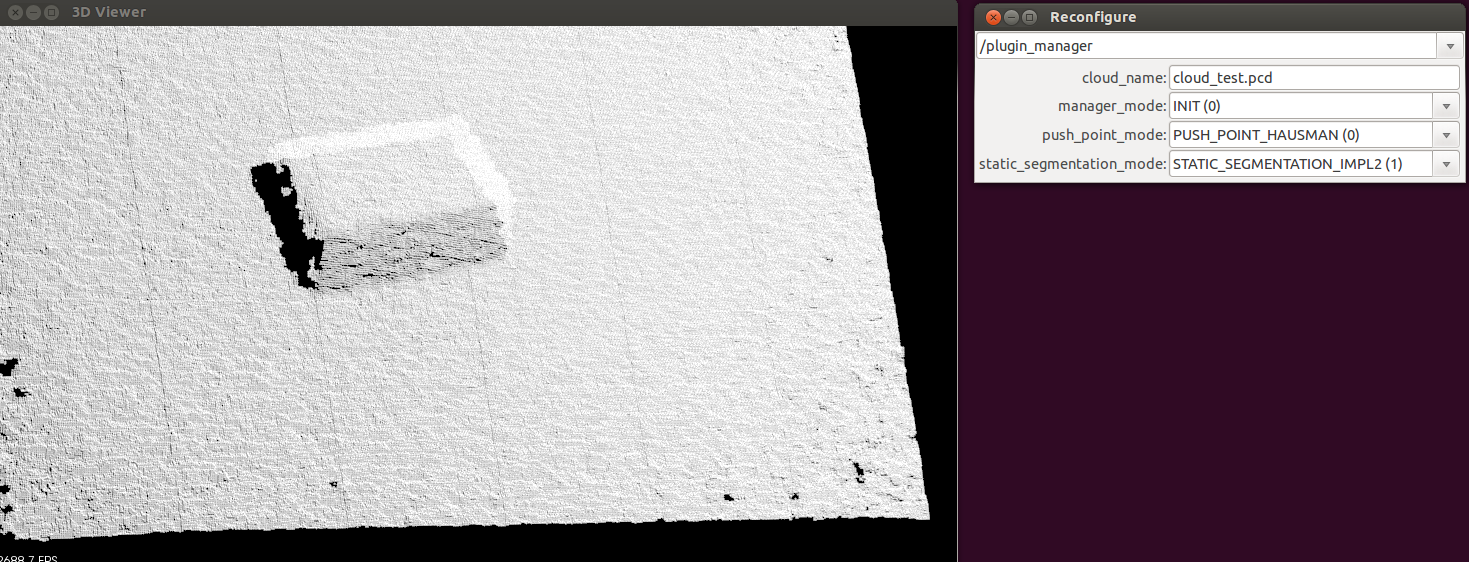
\includegraphics[width=1.1\columnwidth]{figures/ipl.png}}

\caption{Interactive Perception Library with running visualizer and a small Graphical User Interface to choose the step and its implementation.}
\label{fig:ipl}
\end{figure}

The architecture is presented in Fig. \ref{fig:uml}, in the form of an UML class diagram. There is a main class called PluginManager that is responsible for loading different plugins and executing respective steps of the algorithm. It delegates the visualization tasks to the class named Visualizer. The only connection that PluginManager has to the plugins is through the $interactive_perception_interface$ package that consists of all the interfaces for different steps. In addition to that, there are packages responsible for the implementation of the respective step. In Fig. \ref{fig:uml} there are two different implementations for two interfaces - StaticSegmentation and PushPointEstimation. The user can dynamically switch between PushPointImpl and PushPointImpl2 since both of them implement the same generic interface. This design enables other people to benchmark their steps against other algorithms and also to find the combination that fits best to their application.  

\begin{figure}
%\centering
{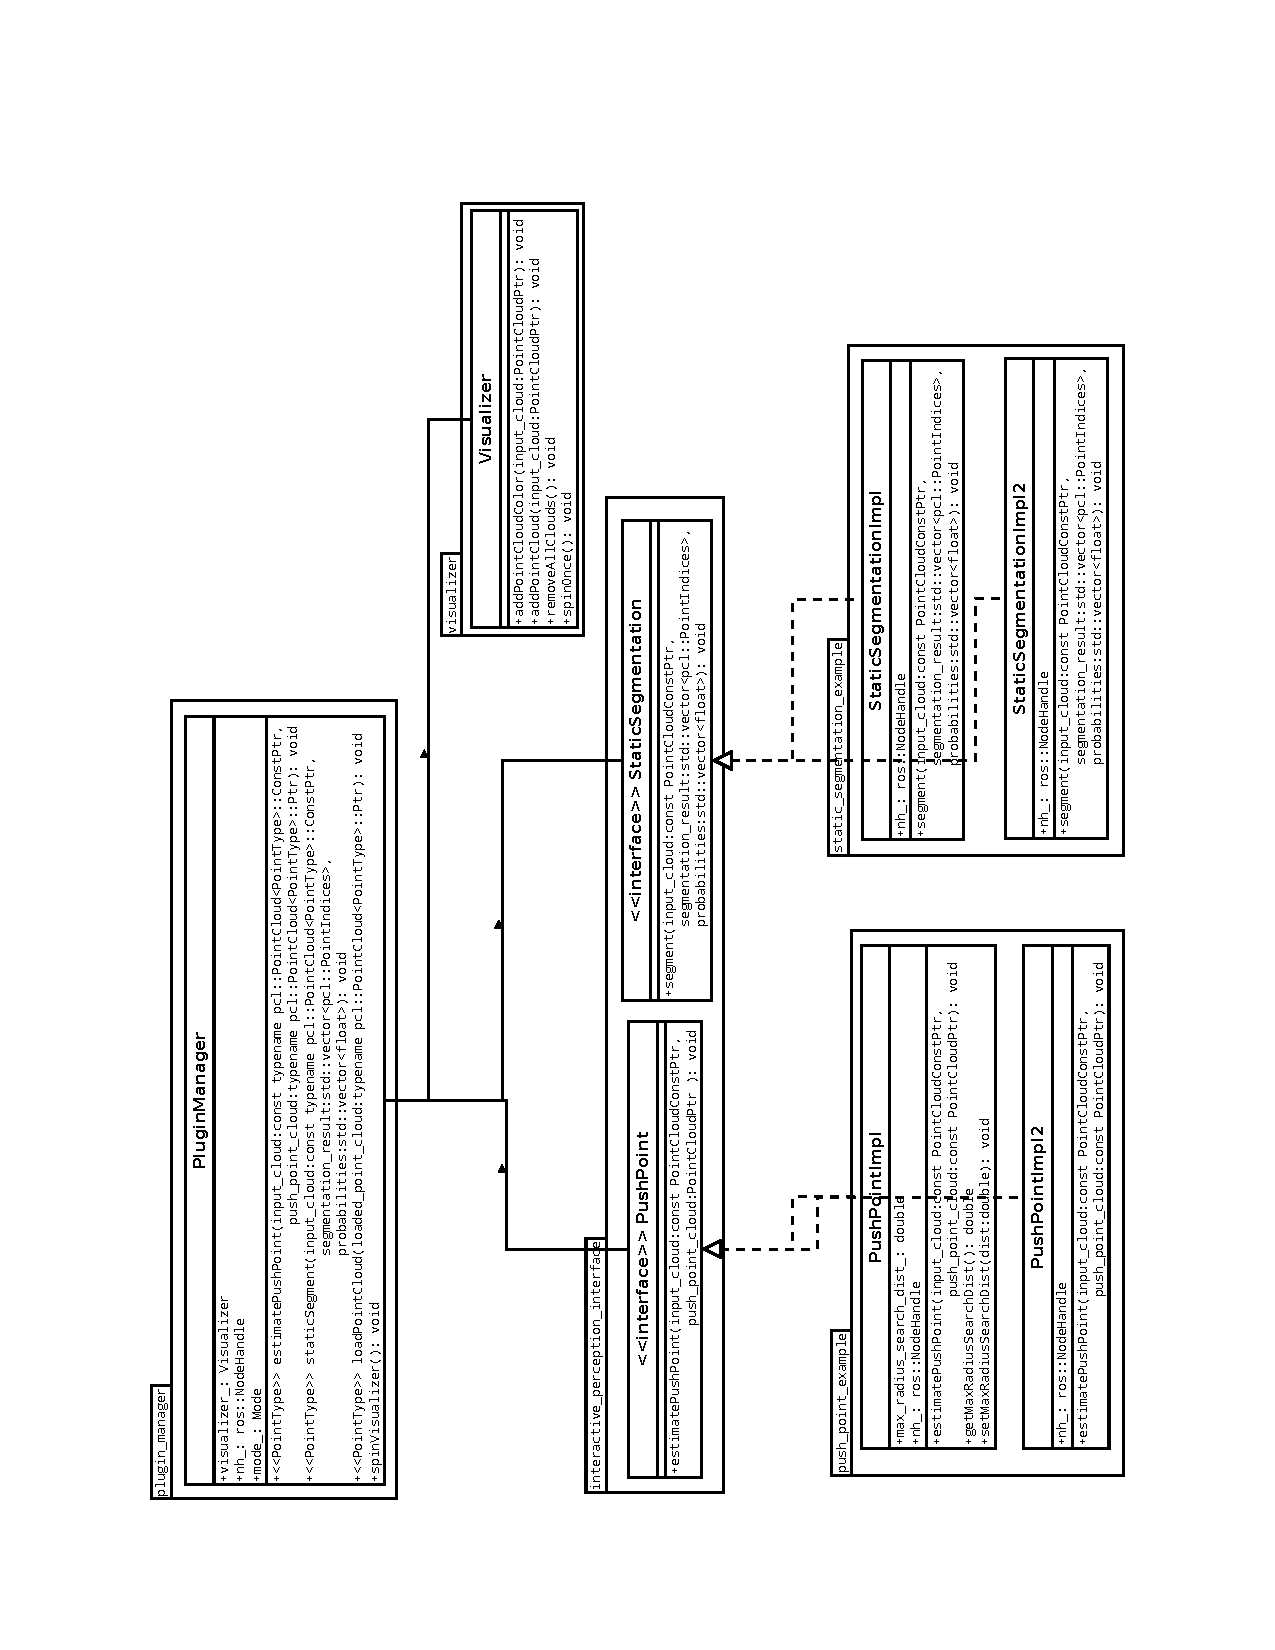
\includegraphics[width=1.1\columnwidth, angle=-90]{figures/uml2.pdf}}

\caption{UML class diagram that shows the main structure of the library.}
\label{fig:uml}
\end{figure}




